The physics modules used are two:

\begin{itemize}
    \item \textbf{Solid Mechanics}: Module used to analyze the mechanical response of the structure to external loading
    \item \textbf{Electrostatics}: Module used to apply electrical charges and analyze the electric field in the structure
\end{itemize}

\noindent
The \textbf{Solid Mechanics} module is used to evaluate the membrane deformation and the resulting von Mises stress under applied pressure. \\
This deformation leads to a change in the capacitance between the membrane and the bottom plate, which can be measured to determine the pressure. \\
To compute this capacitance, a voltage is applied between the diaphragm and the bottom plate, and the \textbf{Electrostatics} module is used to simulate the voltage effect and calculate the capacitance.

\subsection[Solid Mechanics module parameters]{Solid Mechanics module \\ parameters}

All domains are defined as elastic materials, except for the air gap; this means that all domains operate in the elastic regime. \\
The module take the: Young's modulus (\(E\)), Poisson's ratio (\(v\)) and the density (\(\rho\)) from the materials. \\
All boundaries, except for the circular region inside the corrugation of the membrane (where the external pressure is applied, as shown in \autoref{fig:applyed_pressure}), are defined as free. \\
The bottom plate and the lateral border domains are defined with fixed constraints, while the circular region inside the corrugation of the membrane (\autoref{fig:applyed_pressure}) is set as a boundary load with an applied pressure.

\begin{figure}[h!]
    \centering
    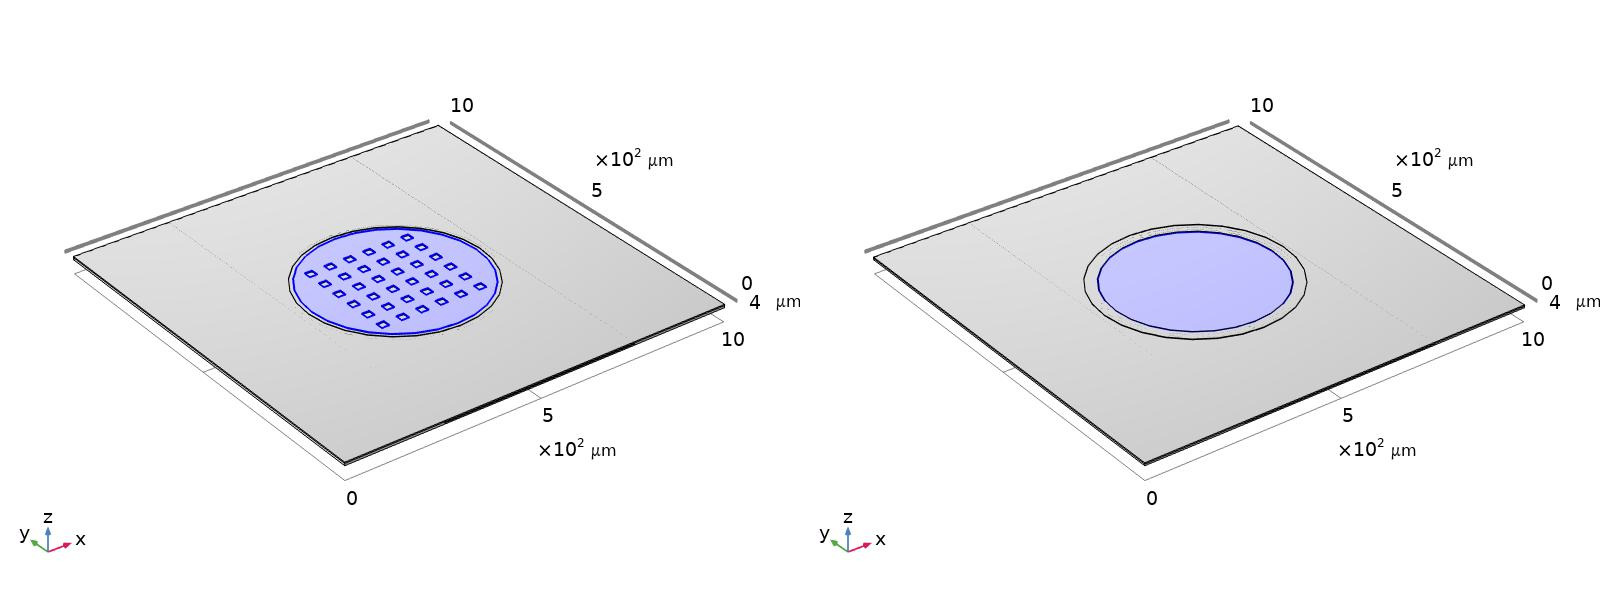
\includegraphics[width=1\linewidth]{img/applyed_pressure.jpg}
    \caption{In both structures, the region where the pressure is applied is highlighted: \\
    left is perforated diaphragm structure, right is perforated back structure}
    \label{fig:applyed_pressure}
\end{figure}

\newpage
\noindent
The initial conditions are the same for all domains, except for the air gap, and set both the initial displacement and the initial structural velocity to zero, as shown in \cref{eq:u=0} and \cref{eq:du/dt=0}.

\begin{equation}
    \vec{u} = (u_x, u_y, u_z) = (0, 0, 0) \; \mu m
    \label{eq:u=0}
\end{equation}

\begin{equation}
    \frac{\partial \vec{u}}{\partial t} = \frac{\partial}{\partial t}(u_x, u_y, u_z) = (0, 0, 0) \; \frac{\mu m}{s}
    \label{eq:du/dt=0}
\end{equation}

\subsection{Electrostatics module parameters}

The air gap domain is defined as free space; this means that, for this domain, the relation in \cref{eq:eps=0} holds.

\begin{equation}
    \epsilon_r = 1 \Rightarrow
    \vec{D} = \epsilon_0 \vec{E}
    \label{eq:eps=0}
\end{equation}

\noindent
All boundaries are defined as zero charge; this means that the charge density on those boundaries is zero, as shown in \cref{eq:rho=0}.

\begin{equation}
    \rho = 0 \; \frac{C}{m^2}
    \label{eq:rho=0}
\end{equation}

\noindent
The internal surface of the bottom plate is connected to ground (\(V = 0 \; V\)), and the diaphragm is defined as a terminal domain with an externally applied potential. \\
For the initial conditions, the potential of both the bottom plate and the diaphragm is set to zero.

\subsection{Multiphysics module parameters}

The \textbf{Multiphysics} module allows different physics interfaces to interact with each other. \\
The feature that enables the interaction between the \textbf{Electrostatics} and \textbf{Solid Mechanics} modules is the \textbf{Electromechanics, Solid} coupling. \\
The only domain selected for this coupling is the diaphragm domain.

\subsection{Mesh construction}

The mesh is automatically generated by COMSOL. \\
The mesh sequence is physics-controlled and defined as extra coarse due to the limited computational resources available on the computer used. \\
The structure is discretized into triangular and tetrahedral elements, and the number of generated entities for both structures is shown in \autoref{fig:mesh_perf_back} and \autoref{fig:mesh_perf_diap}.

\begin{figure}[h!]
    \centering
    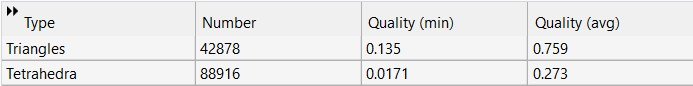
\includegraphics[width=1\linewidth]{img/mesh_perf_back.jpg}
    \caption{Number of mesh entities for the perforated backplate structure}
    \label{fig:mesh_perf_back}
\end{figure}

\begin{figure}[h!]
    \centering
    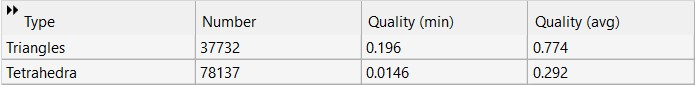
\includegraphics[width=1\linewidth]{img/mesh_perf_diap.jpg}
    \caption{Number of mesh entities for the perforated diaphragm structure}
    \label{fig:mesh_perf_diap}
\end{figure}

\begin{figure}[h!]
    \centering
    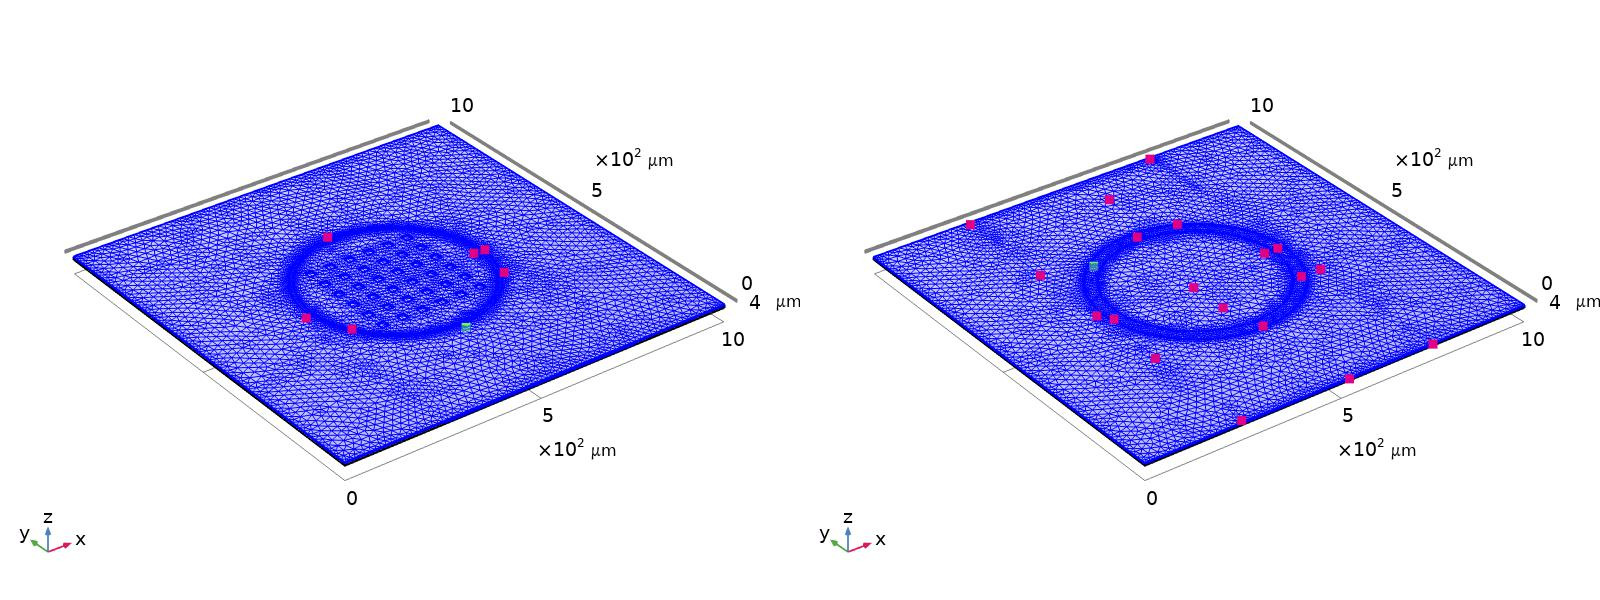
\includegraphics[width=1\linewidth]{img/mesh_build.jpg}
    \caption{Meshed structures: \\
    left is perforated diaphragm structure, right is perforated back structure}
    \label{fig:mesh_build}
\end{figure}